\newslide{Exploring and Searching Signal Presence}{
	\begin{columns}[c]
	\column{0.2\textwidth}
	\begin{tikzpicture}[>=latex',scale=0.4]
	\drawplanexy{-0.3}{-0.3}{-0.3}{6.7}{10}{dashed}{perception}
	
	\drawcube{0}{0}{5}{6.4}{1}{white}{dinamica}{}{};
	\drawcube{0}{1.2}{5}{6.4}{1}{white}{tracking}{}{};
	
	\drawcube{0}{2.4}{5}{6.4}{1}{white}{ostacoli}{}{};
	\drawcube{0}{3.6}{5}{6.4}{1}{white}{altitude}{}{};
	
	\drawcube{0}{4.8}{5}{3}{1.5}{white}{source}{}{};
	\drawcube{0}{6.5}{5}{3}{1.5}{white}{emulatore}{}{};

	\drawplanezy{3.2}{4.8}{5}{4.5}{radar_det}{fill=white,opacity=0.90}{}{};

	\drawcube{3.4}{4.8}{5}{3}{3.2}{gray!40}{alpha}{}{};
	\drawplanexy{-0.3}{-0.3}{5.3}{6.7}{10}{dashed}{action}
	

	\draw [->,line width=1.5] (action_D) -- ++(0,0,2);
	\draw [->,line width=1.5] (perception_D) -- ++(0,0,2);

	\coordinate [at=(radar_det_D), yshift=-5] (arrows_point);
	\draw [->,dashed]  (arrows_point) -- ++(1.5,0,0); 
	\draw [->,dashed]  (arrows_point) -- ++(-1.5,0,0); 
	\end{tikzpicture}
	\vspace{6.5cm}
	\column{0.8\textwidth}
	\begin{block}{}
		\vspace{0.5cm}
		\centering
		Explore the surface, starting from point $\mathbf{p}_0$, to the point $\mathbf{p}_n$

		\vspace{1cm}
		\begin{tikzpicture}[>=latex']
		
			\begin{scope}[xslant=1]
				\draw [ystep=1.5,xstep=3,thin,gray] (0,0) grid (3*3,1.5*3);
				\foreach \x in {1,...,3}
				{
					\foreach \y in {1,...,3} 
					{
						\node at (\x*3-1.5,\y*1.5-0.75) [circle,fill=black,inner sep=1pt] (nodo_\x_\y) {};
						\node [ellipse,draw, minimum width=60, minimum height=30,rotate=0,gray,dashed,xslant=1] at (nodo_\x_\y) {};
					}
				}

				\draw [->] (nodo_1_3) -- (nodo_2_3);
				\draw [->] (nodo_2_3) -- (nodo_3_3);
				\draw [->] (nodo_3_3) -- (nodo_3_2);
				\draw [->] (nodo_3_2) -- (nodo_2_2);
				\draw [->] (nodo_2_2) -- (nodo_1_2);
				\draw [->] (nodo_1_2) -- (nodo_1_1);
				\draw [->] (nodo_1_1) -- (nodo_2_1);
				\draw [->] (nodo_2_1) -- (nodo_3_1);
			\end{scope}
			\node (hexacopter) [at=(nodo_2_3), yshift=50, xshift=10] {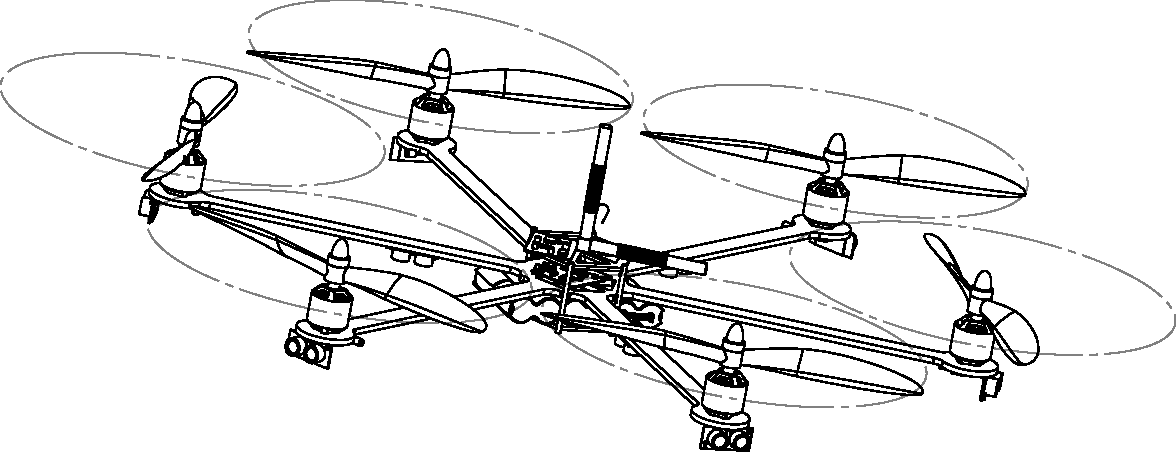
\includegraphics[scale=0.15]{img/hexacopterB.pdf}};
			\coordinate [at=(hexacopter),yshift=-10] (hexapin);
			\draw (hexapin) -- node[pos=1,ellipse,draw=black, minimum width=120, minimum height=70,rotate=0,dashed,xslant=1,fill=gray,opacity=0.4] {} ++(0,-1.5) coordinate(circlecenter);
			\node at (circlecenter) [circle,fill=black,inner sep=1pt] {};
		 	\node [at=(nodo_1_3), yshift=7.5,xshift=7.5] {$\mathbf{p}_0$};
			\node [at=(nodo_3_1), yshift=7.5,xshift=7.5] {$\mathbf{p}_n$};
			\coordinate [at=(nodo_1_3),xshift=-60] (direction1); \coordinate [at=(nodo_1_1),xshift=-60] (direction2);
			\draw [->,line width=2] (direction1) -- node[pos=0.5,above,rotate=45]{Plane direction} (direction2);
			\coordinate [at=(circlecenter),shift=(150:1.3)] (labelA);
			\draw [<-](labelA) -- ++(150:1) -- ++(-2,0) node[above,pos=0.5]{\scriptsize{Receiver range}};

		\end{tikzpicture}
		
		\vspace{1cm}
		We need a strategy to understand if \textbf{there is a signal}
		\vspace{1cm}
	\end{block}
	\end{columns}
}